\subsubsection{Segment Tree (Árvore de Segmentos)}
A Segment Tree é uma estrutura de dados binária que armazena intervalos ou
segmentos. Ela permite realizar consultas de intervalo (como soma, mínimo,
máximo) e atualizações de elementos ou intervalos em tempo $\mathcal{O}(\log
    N)$.

Veja a Segment Tree construída sobre um vetor de 4 elementos:\\ \vspace{0.5cm}
\noindent
\begin{minipage}[t]{0.31\textwidth}
    \centering
    \textbf{Passo 1: Vetor Base}\\
    \vspace{0.2cm}
    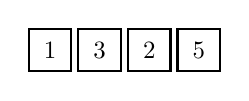
\begin{tikzpicture}[every node/.style={rectangle, draw, minimum size=0.6cm, thick}, scale=0.9, every node/.append style={transform shape}]
        \node (a1) at (0,0) {1};
        \node (a2) at (0.7,0) {3};
        \node (a3) at (1.4,0) {2};
        \node (a4) at (2.1,0) {5};
    \end{tikzpicture}

    \vspace{0.4cm}
    \footnotesize
    \raggedright
    Vetor inicial com 4 elementos ($N=4$).
\end{minipage}%
\hfill
%
\begin{minipage}[t]{0.31\textwidth}
    \centering
    \textbf{Passo 2: Árvore Binária}\\
    \vspace{0.2cm}
    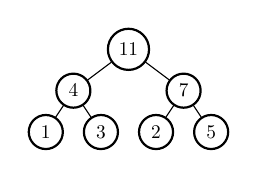
\begin{tikzpicture}[every node/.style={circle, draw, minimum size=0.5cm, thick}, scale=0.7, every node/.append style={transform shape}, >=stealth]
        \node (root) at (1, 1.5) {11};
        \node (l1) at (0, 0.75) {4};
        \node (r1) at (2, 0.75) {7};
        \node (ll) at (-0.5, 0) {1};
        \node (lr) at (0.5, 0) {3};
        \node (rl) at (1.5, 0) {2};
        \node (rr) at (2.5, 0) {5};
        \draw (root) -- (l1);
        \draw (root) -- (r1);
        \draw (l1) -- (ll);
        \draw (l1) -- (lr);
        \draw (r1) -- (rl);
        \draw (r1) -- (rr);
    \end{tikzpicture}

    \vspace{0.2cm}
    \footnotesize
    \raggedright
    Cada nó pai armazena a soma dos filhos (Total = 11, total de 7 nós).
\end{minipage}%
\hfill
%
\begin{minipage}[t]{0.31\textwidth}
    \centering
    \textbf{Passo 3: Atualização}\\
    \vspace{0.2cm}
    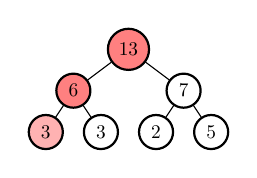
\begin{tikzpicture}[every node/.style={circle, draw, minimum size=0.5cm, thick}, scale=0.7, every node/.append style={transform shape}, >=stealth]
        \node[fill=red!50] (root) at (1, 1.5) {13};
        \node[fill=red!50] (l1) at (0, 0.75) {6};
        \node (r1) at (2, 0.75) {7};
        \node[fill=red!30] (ll) at (-0.5, 0) {3};
        \node (lr) at (0.5, 0) {3};
        \node (rl) at (1.5, 0) {2};
        \node (rr) at (2.5, 0) {5};
        \draw (root) -- (l1);
        \draw (root) -- (r1);
        \draw (l1) -- (ll);
        \draw (l1) -- (lr);
        \draw (r1) -- (rl);
        \draw (r1) -- (rr);
    \end{tikzpicture}

    \vspace{0.2cm}
    \footnotesize
    \raggedright
    Atualiza a posição 0 de 1 para 3. Propaga os valores em $\mathcal{O}(\log N)$.
\end{minipage}

\vspace{0.3cm}

\paragraph{Implementação: }\mbox{}\\
\textbf{C++:}
\begin{lstlisting}[language=C++]
struct SegTree {
    int n;
    vector<long long> tree;

    SegTree(int n) : n(n), tree(4 * n, 0) {}

    void update(int node, int start, int end, int idx, long long val) {
        if (start == end) {
            tree[node] = val;
            return;
        }
        int mid = (start + end) / 2;
        if (idx <= mid) update(2 * node, start, mid, idx, val);
        else update(2 * node + 1, mid + 1, end, idx, val);
        tree[node] = tree[2 * node] + tree[2 * node + 1];
    }

    long long query(int node, int start, int end, int l, int r) {
        if (r < start || end < l) return 0;
        if (l <= start && end <= r) return tree[node];
        int mid = (start + end) / 2;
        return query(2 * node, start, mid, l, r) + query(2 * node + 1, mid + 1, end, l, r);
    }
};
\end{lstlisting}
\newpage